
\chapter{Infrastructure Design}
\label{chap:2}
\section{Infrastructure Designing Overview.}
Infrastructure design involves systematic planning, creation, and optimization of the underlying framework that supports various systems, processes, and activities within an organization or community. Whether it's physical, digital, or social infrastructure, effective design is essential for ensuring functionality, efficiency, scalability, and resilience. Here are key aspects to consider when designing infrastructure.
Infrastructure design begins with thorough planning, involving the identification of needs, goals, and potential challenges. This stage lays the groundwork for the entire design process.
Creation involves the actual construction or implementation of the infrastructure based on the established plans. This includes selecting appropriate technologies, materials, and methodologies to bring the design to life.
Optimization is an ongoing process aimed at enhancing the efficiency, performance, and effectiveness of the infrastructure. This may involve fine-tuning processes, upgrading equipment, or implementing new technologies to improve overall. 
Infrastructure design should cater to the diverse needs of different systems, processes, and activities within the organization or community. This entails ensuring compatibility, integration, and seamless operation across various components.
The primary goal of infrastructure design is to ensure that it functions as intended, providing reliable support for the activities it is designed to facilitate. This includes considering factors such as usability, accessibility, and reliability.
Efficiency is a key consideration in infrastructure design, aiming to optimize resource utilization and minimize waste. This may involve streamlining processes, adopting energy-efficient technologies, or implementing automation where possible.
Infrastructure should be designed with scalability in mind, allowing for expansion or contraction as needed to accommodate changes in demand or growth. This may involve designing modular systems or incorporating flexible architecture.
Resilience is essential for ensuring that infrastructure can withstand and recover from disruptions or adverse conditions. This may involve building redundancy, implementing disaster recovery plans, or enhancing security measures to mitigate risks. \cite{DSR}



\section{ Hybrid Mail Solution Infrastructure Design with Data Center Disaster Recovery (DCDR)}
\begin{figure}[!htb]
    \centering
    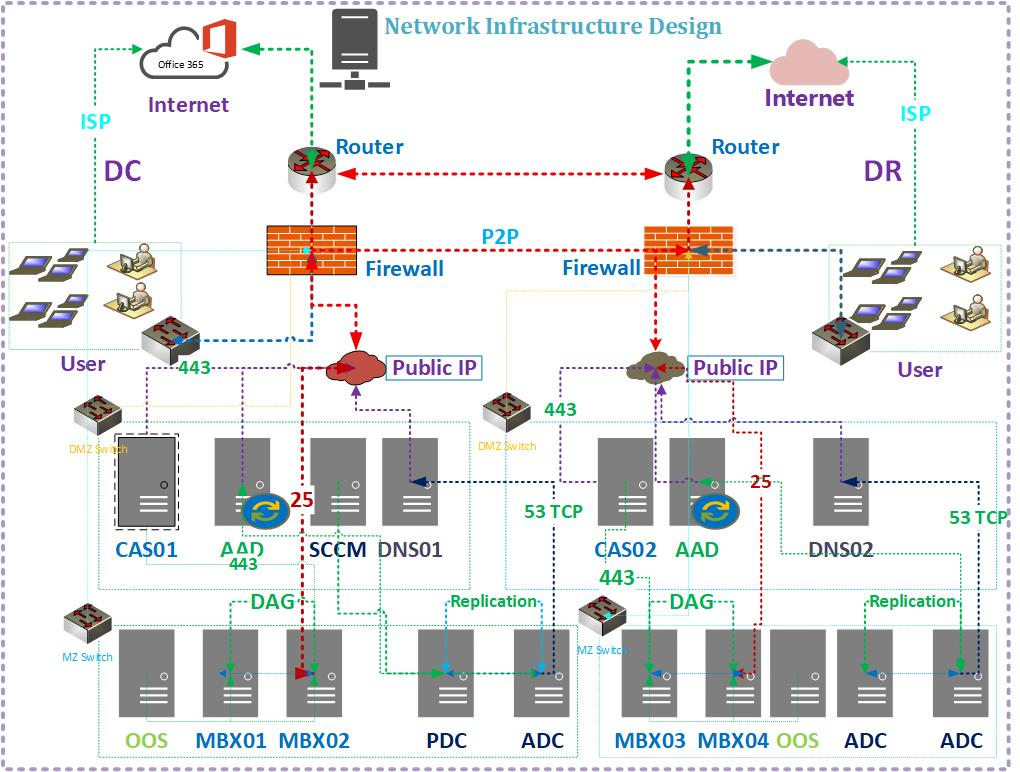
\includegraphics[scale=0.5]{Chap2/Network Infrastructure Design.jpg}
    \caption{Network Infrastructure design}
    \label{fig:my_label}
\end{figure}

\section{Design Objectives}
\begin{itemize}
    \item According to the above- mentioned Hybrid Mail Solution Infrastructure Design with Data Center Disaster Recovery (DCDR), a total of four Active Directory servers—two per datacenter—are used for redundancy.
    \item A total of four mailbox servers using DAG (Database Availability Group) replication for redundancy are present across the two datacenter.
    \item In accordance with security best practices, all Active Directory and Mailbox Servers, including the optional Office Online Server, will be installed on the Server Firm Zone Network.
    \item The only reason  need a proxy is to enable SSL URLs for SSL Revocation Pass on Mailbox since these servers won't have access to the internet.
    \item The Mailbox Server's public static IP port must be forwarded via IronPort [Anti-Spam Gateway, Ports 25 Inbound and Outbound] and Reverse Proxy [Mailbox CAS (Client Access Server) Gateway, Port 443 Inbound] on the DMZ Zone where  will need direct internet access.
    \item In order to protect Active Directory from direct internet exposure, I have also set up a Public Facing DNS server that will resolve public domain names for Mailbox and Active Directory integrated DNS by using a DNS forwarding rule on Active Directory integrated DNS.
    \item In order to perform manual failover in the event that the DC Datacenter goes down, I can configure the Primary Witness on Active Directory Server in the DC Datacenter and an Alternate Witness on Active Directory in the DR Datacenter. 
    \item Placing the Witness server for Mailbox Server auto Failover on a third location is optional if a third location cannot be arranged.
    \item Business Continuity with seamless failover and disaster recovery capabilities for messaging services.
    \item Hybrid Coexistence enabling secure mail flow, free/busy sharing, and mailbox migration between on‑premises and Exchange Online.
    \item Modern Authentication & Security aligned with Microsoft best practices for identity, encryption, and compliance. \cite{mahmud_brain-inspired_2018,8742551,noauthor_coronavirus_nodate}
    
\end{itemize}
